\documentclass[tikz,border=1pt]{standalone}
\usepackage[T1]{fontenc}
\usepackage{helvet}
\renewcommand{\familydefault}{\sfdefault}
\usepackage{tikz}
\usetikzlibrary{arrows.meta,positioning,calc}
\definecolor{ink}{HTML}{1F2933}
\definecolor{line}{HTML}{52606D}
\definecolor{panel}{HTML}{F5F7FA}
\definecolor{network}{HTML}{0E7490}
\definecolor{power}{HTML}{B45309}
\definecolor{store}{HTML}{475569}
% Single-column layout, used at 100% scale in main.tex (Fig. 1).
% Left column: host, storage, supply. Right column: switch, Pi, meter.
% Every arrow label sits in empty space; no arrow crosses a box.
\begin{document}
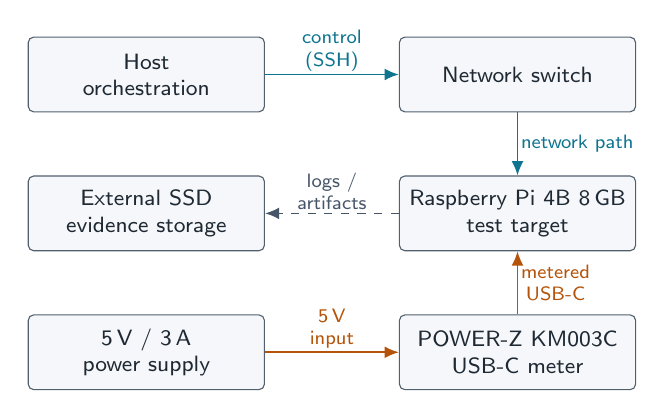
\begin{tikzpicture}[
  font=\sffamily\footnotesize,
  box/.style={draw=line,fill=panel,rounded corners=2pt,minimum width=30mm,
              minimum height=9.5mm,align=center,text=ink,inner sep=1.5pt},
  arr/.style={-{Latex[length=1.8mm,width=1.5mm]},line width=.6pt},
  lab/.style={font=\sffamily\scriptsize,align=center,inner sep=1pt}
]
% right column (device-under-test path)
\node[box] (sw)    at (0,0)              {Network switch};
\node[box] (pi)    [below=8mm of sw]     {Raspberry Pi 4B 8\,GB\\test target};
\node[box] (meter) [below=8mm of pi]     {POWER-Z KM003C\\USB-C meter};
% left column
\node[box] (host)  [left=17mm of sw]     {Host\\orchestration};
\node[box] (ssd)   [left=17mm of pi]     {External SSD\\evidence storage};
\node[box] (psu)   [left=17mm of meter]  {5\,V / 3\,A\\power supply};

% network / control (teal)
\draw[arr,network] (host) -- node[lab,above,text=network]{control\\(SSH)} (sw);
\draw[arr,network] (sw)   -- node[lab,right,text=network]{network path} (pi);
% evidence storage (grey, dashed)
\draw[arr,store,dashed] (pi) -- node[lab,above,text=store]{logs /\\artifacts} (ssd);
% power measurement (amber)
\draw[arr,power] (psu)   -- node[lab,above,text=power]{5\,V\\input} (meter);
\draw[arr,power] (meter) -- node[lab,right,text=power]{metered\\USB-C} (pi);
\end{tikzpicture}
\end{document}
